% Author: Izaak Neutelings (March 2021)
% page 8 https://archive.org/details/StaticAndDynamicElectricity
% https://tex.stackexchange.com/questions/56353/extract-x-y-coordinate-of-an-arbitrary-point-on-curve-in-tikz
% https://tex.stackexchange.com/questions/412899/tikz-calculate-and-store-the-euclidian-distance-between-two-coordinates
\documentclass[border=3pt,tikz]{standalone}
\usepackage{amsmath} % for \dfrac
\usepackage{mathabx} % for \Earth
\usepackage{bm} % \bm
\usepackage{physics}
\usetikzlibrary{3d}
\usepackage{tikz,pgfplots}
\usepackage[outline]{contour} % glow around text
\usepackage{ifthen}
\usetikzlibrary{calc}
\usetikzlibrary{intersections}
\usetikzlibrary{decorations.markings}
\tikzset{>=latex} % for LaTeX arrow head
\pgfplotsset{compat=1.13}
\contourlength{1.2spt}
\usepackage{xcolor}
\colorlet{Ecol}{orange!90!black}
\colorlet{EcolFL}{orange!80!black}
\tikzstyle{charge+}=[very thin,top color=red!50,bottom color=red!90!black,shading angle=20]
\tikzstyle{charge-}=[very thin,top color=blue!50,bottom color=blue!80,shading angle=20]
\tikzset{EFieldLine/.style={thick,EcolFL,decoration={markings,mark=at position #1 with {\arrow{latex}}},
                                 postaction={decorate}},
         EFieldLine/.default=0.5,
         EFielLineArrow/.style args = {#1}{EcolFL,decoration={markings,
          mark=at position 0.5 with {\arrow[rotate=#1]{latex}}},
          postaction={decorate}}
}


\makeatletter
  \newcommand{\xy}[3]{% % FIND X, Y
    \tikz@scan@one@point\pgfutil@firstofone#1\relax
    \edef#2{\the\pgf@x}%
    \edef#3{\the\pgf@y}%
  }
\makeatother
\newcommand{\EFielLineArrow}[2]{ % ELECTRIC FIELD LINE ARROW
  \pgfkeys{/pgf/fpu,/pgf/fpu/output format=fixed} % for calculation between -1*10^324 and +1*10^324
  \pgfmathsetmacro{\x}{#1/28.45pt}
  \pgfmathsetmacro{\y}{#2/28.45pt}
  \pgfmathsetmacro{\U}{\Q*((\x+\a)^2+(\y)^2)^(3/2)}
  \pgfmathsetmacro{\V}{\q*((\x-\a)^2+(\y)^2)^(3/2)}
  \pgfkeys{/pgf/fpu=false}
  \pgfmathparse{
    atan2(((\y)*\V+(\y)*\U),((\x+\a)*\V+(\x-\a)*\U))
  }
  \edef\angle{\pgfmathresult}
  \pgfmathsetmacro{\D}{int(1000*\q*(\x+\a)/sqrt((\x+\a)^2+\y*\y) + 1000*\Q*(\x-\a)/sqrt((\y-\a)^2+\y*\y))/1000}
  \draw[EFielLineArrow={\angle}] (\xpt,\ypt);
}
\newcommand{\EFieldLines}{ % ELECTRIC FIELD LINES
  \message{^^JField lines (\q,\Q) with contours range ^^J\range^^J}
  
  % FIELD LINES
  \draw[EcolFL,name path=Elines] plot[id=plot, raw gnuplot, smooth]
    function{
       f(x,y) = \q*(x+\a)/sqrt((x+\a)**2+y**2) + \Q*(x-\a)/sqrt((x-\a)**2+y**2);
       set xrange [-\xmax:\xmax];
       set yrange [-\ymax:\ymax];
       set view 0,0;
       set isosample 400,400;
       set cont base;
       set cntrparam levels discrete \range;
       unset surface;
       splot f(x,y)
    };
  
  % ELLIPSE INTERSECTIONS
  \path[name path=ellipse1] (\a,0) ellipse ({0.8*\R} and {1.3*\R});
  \message{Intersections...}
  \path[name intersections={of=Elines and ellipse1,total=\t}]
    \pgfextra{\xdef\Nb{\t}};
  \message{ found \Nb ^^J}
  \foreach \i in {1,...,\Nb}{
    \message{  \i}
    \xy{(intersection-\i)}{\xpt}{\ypt}
    \EFielLineArrow{\xpt}{\ypt}
    \message{ (\D,\x,\y)^^J}
  }
}
\newcommand{\EFieldLinesDashed}{ % ELECTRIC FIELD LINES
  \message{^^JField lines (\q,\Q) with contours range ^^J\range^^J}
  \draw[EcolFL,dashed] plot[id=plot, raw gnuplot, smooth]
    function{
       f(x,y) = \q*(x+\a)/sqrt((x+\a)**2+y**2) + \Q*(x-\a)/sqrt((x-\a)**2+y**2);
       set xrange [-\xmax:\xmax];
       set yrange [-\ymax:\ymax];
       set view 0,0;
       set isosample 400,400;
       set cont base;
       set cntrparam levels discrete \range;
       unset surface;
       splot f(x,y)
    };
}


\begin{document}


% CHARGE IMAGE - SPHErE
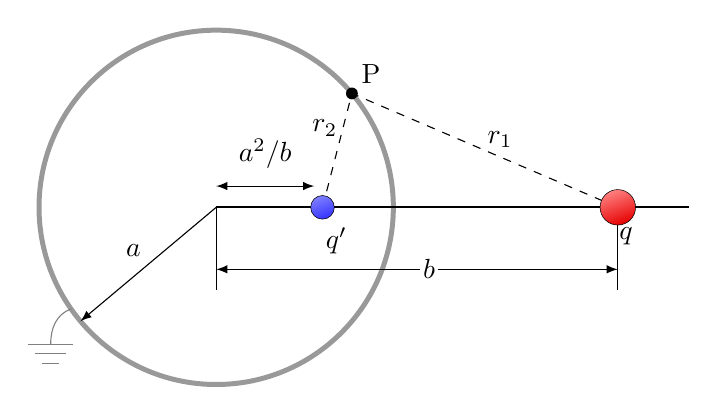
\begin{tikzpicture}[scale=1.5]
  \def\R{1.5}
  \def\L{4.0}
  \coordinate (Q') at (0.6*\R,0);
  \coordinate (Q) at (0.85*\L,0);
  \coordinate (A) at ({\R*cos(40)},{\R*sin(40)});
  
  \draw[] (Q) -- ++ (0, -0.7);
  \draw[] (0,0) -- ++ (0, -0.7);
  % SPHEREs
  \draw[black!40,line width=1.8] (0,0) circle(\R);
  \draw[black!50,line cap=round]
    (-145:\R) to[out=-160,in=90]++ (-120:0.23*\R) coordinate (G);
  \foreach \i [evaluate={\y=(1-\i)*0.08; \w=0.5*(0.5-\i*0.12);}] in {1,2,3}{
    \draw[black!50]
      (G)++(-\w,\y) --++ (2*\w,0);
  }
  
  % AXES
  \draw[thick] (0,0) -- (\L,0); %node[below left=-2] {$x$};
  \draw[->] (0,0) -- (-140:\R) node[thick, midway,above left=-1] {$a$};
  
  % CHARGE
  \draw[dashed] (Q') -- (A) node[pos=0.6,above left=-2.5] {$r_2$};
  \draw[dashed] (Q) -- (A) node[pos=0.5,above right=-2.5] {$r_1$};
  \fill (A) circle (0.05) node[above right=0] {P};
  \draw[charge+] (Q) circle (0.15) node[right=3,below=4] {$q$};
  \draw[charge-] (Q') circle (0.10) node[right=5,below=4] {$q'$};
  %\draw[<->] ([yshift=-8]Q') -- ([yshift=-8]Q)
  %  node[midway,fill=white,inner sep=1] {$d$};
  
  \draw[<->] (Q)++(0,-0.35*\R) -- (0,-0.35*\R)
    node[pos=0.47,fill=white,inner sep=1] {$b$};
  \draw[<->] (Q')++(-0.07,0.12*\R) -- (0,0.12*\R)
    node[midway,above=5, fill=white,inner sep=1] {$a^2/b$};
  
\end{tikzpicture}



\end{document}